\documentclass{article}
\usepackage{graphicx} % Required for inserting images
\usepackage{float}
\usepackage{booktabs}
\usepackage[skip=10pt, indent=0pt]{parskip}
\bibliographystyle{acm}

%\title{Predicting Snakebite Incidence In Brazil Under Different Climate Change Scenarios}
\title{A statistical modelling framework for scenario-based forecasting of health outcomes}
\author{Matt Timperley 
\and 
Emanuele Giorgi
}
\date{}

\begin{document}

\maketitle

%\section{Introduction}

% Prantivenom
    % Snakebites bad - burden etc (could put this elsewhere) - mention NTD? see \cite{pintor_addressing_2021}
    % anitvenom drawbacks i.e. stockpiling
    % wrong type in area / not enough / wrong type / developed for snakes not in that region for partial effectiveness. 
    % Might mention upcoming drug alternatives to antivenom (optional, that fella we chatted to)
    % same drawbacks presant
    % under reporting / not seeking medical care

% Problem continued - problems with approach
% difficulties with snakebite prediction - changing environment and land use etc plus inherant glrowing uncertainty of prejections esp when predicting based off other predictied values as with lagged data.
    % environment change + land use
    % changes habitat = move
    % or changes prey habitat = move
    % cold blooded, sensitive to environment, change to env = move
    % can also affect behaviour making bit more likely
    % swiss cheese model - look at boundaries.
    
    % climate change effects snake distribution - cold blood, temperature, rainfall, breeding, aggression etc.
    % human activity intertwined - farming in particular provide abundant food for snake-edible things. more contact with humans, 
    % swiss cheese model paper reference - Highlight overlap in snakes and humans. I think we can assume that all snakes bite for the sake of pressure. although there are constrictor species and harmless bites. So species plays a role.

% Objectives - how we will address the issues
    % predicting snakebite incidence over space and time so that treatment can be stockpiled when and where will be most effective. sexy tag line.

% Related works
    % other climate change mapping papers may be relevant. Put them here. - at least V. Pitzer
    % Joacim similar framework - differences and novelty
    % other snakebite risk-mapping studes. Perhaps a table of times / location / S-T-ST models to show where we fit in terms of that novelty
    
% round up and give the remaining structure of paper.




% nomenclature
% i - locations in space
% y - locations in time
% n_t total locations in time
% n_i total locatoins in space
% y number of snakebites, modified by i / t



\section{Framework}

% In this section - rewrite this paragraph for the full paper
We will elaborate on the proposed framework by first presenting a visual depiction, as shown in Figure \ref{fig:framework}, followed by a thorough explanation. This framework delineates a series of sequential steps aimed at harnessing initial disease data to generate pertinent outputs. To elucidate the efficacy of this framework, we will delve into a case study focusing on snakebites in Brazil spanning from 2007 to 2020.

Snake envenoming, being a consequence of interactions between humans and their environment, epitomizes an environmental disease with profound public health implications. Its occurrence is intricately linked to ecological factors such as habitat encroachment, climate change, and land use patterns, underscoring the importance of understanding its spatio-temporal dynamics within a broader environmental context. This emphasizes the significance of employing robust methodologies capable of capturing the intricate interplay between environmental variables and disease transmission dynamics.

Moreover, the versatility of the outlined methodology extends beyond the realm of snakebites to encompass a diverse array of infectious diseases. From mosquito-borne illnesses like malaria and dengue fever to waterborne pathogens such as cholera and leptospirosis, the framework provides a systematic approach for analyzing and understanding the complexities of disease transmission dynamics. By integrating environmental data, epidemiological parameters, and demographic factors, this methodology enables a comprehensive examination of disease dynamics, facilitating informed decision-making in disease control and prevention efforts. Thus, while the initial focus may be on snakebites, the methodology's broader applicability underscores its potential as a valuable tool in combating a wide spectrum of infectious diseases worldwide.

\begin{figure}[h!]
    \centering
    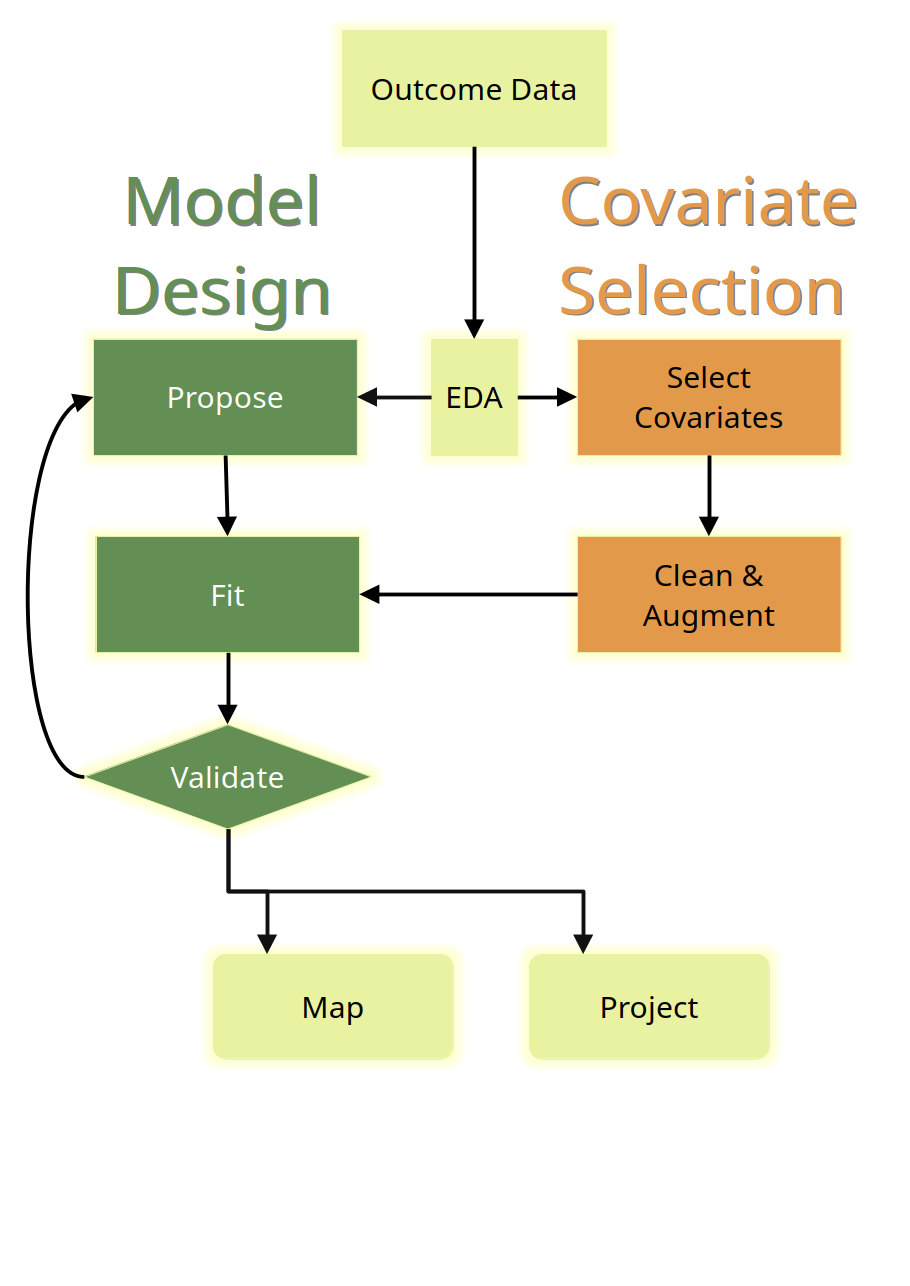
\includegraphics[scale=0.22]{images/process flow.png}
    \caption{"A flow chart of the proposed framework"}
    \label{fig:framework}
\end{figure}


% overview and graph - explaining the whole framework from disparate data sources to usable dataset
The framework can be conceptualised as an iterative refinement of the Box-Jenkins process, akin to its application in \cite{jereModellingEpidemiologicalData2016}. However, it distinguishes itself by introducing a more formalised initial model proposal. Furthermore, it extends its scope beyond the traditional ARIMA models by incorporating considerations for various external factors. This generalised approach facilitates the adaptation of diverse modelling techniques tailored to specific disease dynamics.

In addition to model development, the framework integrates a comprehensive data processing component, ensuring the seamless transformation of raw data into actionable insights. 



\subsection{Outcome Data}
% Data - where from, basic overview
The framework exists to structure the analysis of data regarding a particular outcome. This could be from a number of potential sources, such as prevalence data from surveys, or notified cases from a health authority. In our example we obtained notified case data for the whole of Brazil from 2007 to 2020.

In addition to the outcome data itself, some form of spatial and/or temporal location is required. This may require additional processing to be usable. For example, in the case where street addresses are given with the outcome, geocoding can be used to assign spatial coordinates to the data. Open Street Map (OSM) \cite{osm} is a resource which can be used for geocoding.
% sinan human cases
The snakebite data assigned a number of cases on a given date to a municipality. This will impact the model design as our data is areal in nature, which makes models based on the distance between points inappropriate. This is one of a number of preprocessing steps required to convert the data into a form appropriate for modeling. The specifics are dictated by the data set in question.

% agg to monthly regional - why then how
The snakebite data was aggregated to monthly cases per region, based on a lookup table of region IDs and municipality IDs. The monthly aggregation was performed by processing the date. It is worth noting that the spatial IDs are chosen to match with shape files for Brazil. Having this link is useful for both further processing and for visualisation, for areal data. Point data can be readily used without this concern, replaced instead with the requirement that all resources share a matching projection e.g. WGS-84.

Common preprocessing steps include: converting from one file format to another, aggregating over space or time, converting between data types, or merging data from additional sources. These could be satellite data from images, census data from other files, or data derived from existing values. The additional data should include the candidates for becoming model covariates.

% processing types (dates, numbers, coords as strings for matching to avoid rounding inequalities, or as numbers for ordering i.e. remove coords < 11.5 lat
A very common part of processing data is converting between types. Most programming languages have a number of date types available through libraries and leveraging this can be extremely useful. Converting between strings and numbers is also common.
% geolocation - osm for address to wgs84 (or other csm)
Geolocation is the process of assigning coordinates to addresses. These coordinates will be projected in a particular way which must match across the analysis. Geolocation can be a good example of when it may not be obvious what type to use. For matching locations it is useful to use a string representation as it retains parity. Numerical representations of coordinates can be rounded and no longer match. This becomes a concern where an index of addresses is geolocated, then used as a lookup table to apply to the original data. However, the requirements reverse where filtering occurs i.e. to remove coordinates outside of a range is far easier using a numeric representation.

In the snakebite example no geolocation was required as the outcome data was already assigned a municipality and region ID. This also has an impact on our initial model proposal. Namely, the data is areal in nature and, without additional processing to point locations, the model will need to account for this.

% the power of nothing
Zeroes can also be an important point to consider. There is a distinct difference between zeroes which represent unknown results, and those which represent a negative survey \cite{andersonBlackSwansSpace2019}. The model will need to account for this too, as will the interpretation of results.

% data constrints suggest initial model
The nature of the outcome data gives an indication of where to start when modeling. An exploratory data analysis (EDA) is useful for finding these insights as well as discovering additional constriants. The most basic element is to consider the distribution and nature of the outcome. In the case of the snakebite data, these are notified cases from hospitals across municipalities in Brazil. These have an undereporting issue, as is the case in many countries \cite{chavesSnakebitesAreAssociated2015} \cite{ediriweeraHealthSeekingBehavior2017}. Only the severe bites, favouring different species, and people who have willingness and availability to visit a hospital are biased towards. Notified cases are not part of a wider survey, so nothing is known about test coverate, which suggests our model will have a Poisson outcome in the case of our snakebite example.

We can consider the world of potential linear models as ranging from the least complex, simply an intercept, to the infinitely complex. It is important to strive for model parsimony. Sensible models in our case range from a linear combination of covariates, weights and an intercept, up to spatio-temporal models.

Autocorrelation gives us insights as to whether adding a spatial or temporal component would allow our model to explain more of the variance. Where there are spatial or temporal residuals, we should account for this as we develop our model.

% look for spatial autocorrelation
Spatial autocorrelation can be shows by examining autocorrelation residuals at different distance lags. The residuals are taken after fitting a model which removes other covariates, such that just the assumed spatial effects remain. One expects that if a spatial relationship exists, that points closer to one another in space are more similar than those further apart. This results in a characteristic curve. We can see this by plotting the empirical variogram. Note that the data here has been aggregated over time, such that each spatial location has only one count. The empirical variogram of snakebite cases can be seen in Figure \ref{fig:varioverview}. The residuals were taken from a simple intercept model, on just the outcome data as a first step: $y_i = \alpha$ The curve in the figure is a model with a Matern spatial effect.

\begin{figure}[h]
    \centering
    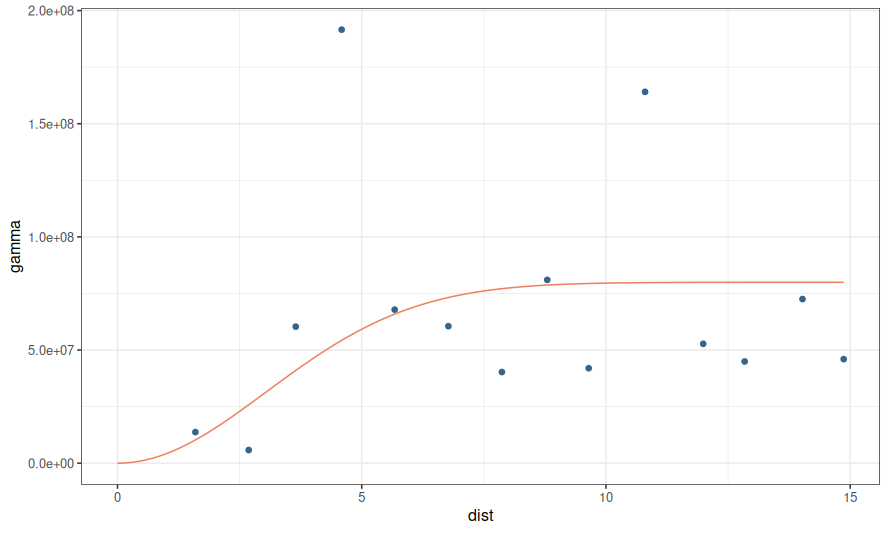
\includegraphics[scale=0.5]{images/varioverview.png}
    \caption{ACF plot of snakebite cases collapsed over space.}
    \label{fig:varioverview}
\end{figure}

% evidence of temporal effects
The autocorrelation function (ACF) indicates patterns between the variable of interest with itself at various time lags. Where the values lie outside of the 5\% confidence band, this indicates a temporal pattern in the variable. The ACF plot for the snakebite cases is given in Figure \ref{fig:acfoverview}. As this is an analysis of time, the outcome (number of bites) is collapsed over space i.e. the number of bites is aggregated such that there is a single count per time t.

\begin{figure}[h]
    \centering
    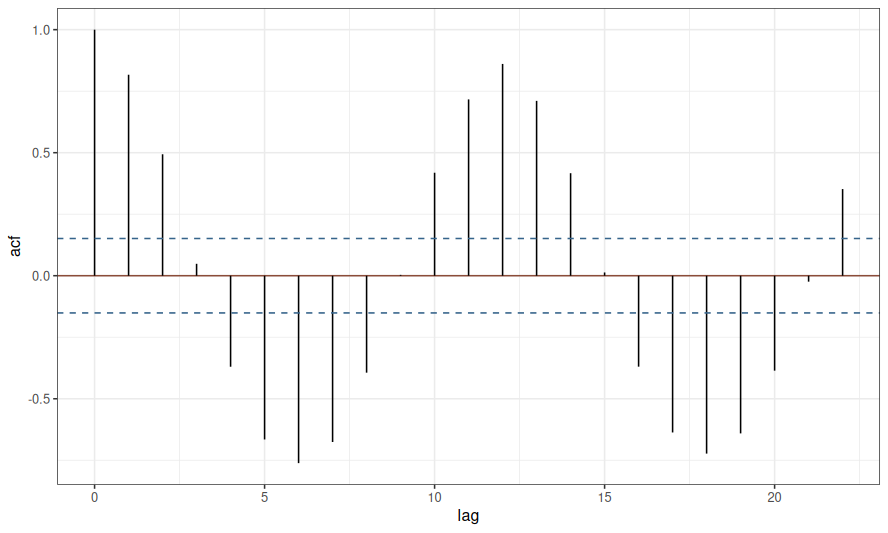
\includegraphics[scale=0.5]{images/acfoverview.png}
    \caption{ACF plot of snakebite cases collapsed over space.}
    \label{fig:acfoverview}
\end{figure}

% round up / link sentence
As we can see from Figures \ref{fig:acfoverview} and \ref{fig:varioverview}, there is evidence of both spatial and temporal elements in the outcome data. At this stage we can conclude that we will need to include both aspects in our model. However, instead of proceeding to an initial model we must first consider the covariates which we will include in our model. These covariates may already account for spatial or temporal autocorrelation which can significantly alter the model we will design.

\subsection{Covariate Data}

The first step is to identify useful covariates. This could be done in a number of ways. For example, a data mining approach would have many potential covariates and then select those which have the greatest power to predict the observed outcome data. This approach may not give results which generalise well to other situations, because the choices were not driven by an understanding of the biological reality of the situation. This can lead to a lack of parsimony thereby and overspecialisation. In the snakebite example we chose covariates using expert knowledge, i.e. from relevant literature. Less well explored scenarios may require more direct expert input or some combination of techniques.

% covariates from literature 
    % look at x different geographic reagions
    % covs from Sri Lanka
    % covs from costa rica
    % covs from Brazil - strong agri \cite[mise_agriculture_2016]
    % Need to add Africa - add to lit review

% environmental from isimip - data aug. TODO: mention the other land use and socio are included through choice of ssp rcp
We identified 3 relevant environmental covariates from the literature: Temperature, rainfall and humidity. These were obtained from the ISIMIP website, using bias-adjusted atmospheric climate input data \cite{10.48364/ISIMIP.208515}. Data sources can also be influenced by a number of factors. In the case of the snakebite data, the research questions being addressed required some inclusion of socioeconomic and land use factors, as well as projections into the future. ISIMIP provides data fitting these criteria.

% taking from different inputs (excel, csv, netcdf, geotiff, geojson, shapefile) - quick note on data types
Additional data may come in a variety of formats that require conversion. comma separated variable (CSV) files are a simple and clean format which we adopted for intermediate steps and outputs. Excel files require conversion using libraries as they contain a lot of unnecessary data and potentially multiple sheets. Outcome data and census data can often be in this format initially. This is all for tabular data. The other common format is based around images. GeoTIFF and shapefiles both store raster/vector data, which shows data as an image an represents a single point in time, usually. NetCDF is an alternative to having a number of image files over a span of time, instead storing spatio-temporal data in a single file. A comprehensive index and meta-data structure sit around the single array of data spanning all space and time coordinates, more information can be found in \cite{singhEfficientNetCDFProcessing}.

Regardless of format, the data is processed and sampled to add potential covariates to the outcome data. In the case of environmental covariates obtained from ISIMIP, these are netCDF. The boundries of Brazil and its regions can be obtained in several formats from the Database of Global Administrative Areas (GADM) \cite{gadmDatabaseGlobalAdministrative}.

% EDA insights
An initial EDA gives some insights into how we should process our covariates. We can look for correlation between covariates to see if any are redundant. We can compare the scales and distributions to suggest a need for normalisation or standardisation. In this case, the covariates do have some correlation, but all remain distinct enough that they were all included. % TODO: come back to this in iterative evaluation, testing best fitting models.

% adding covariates to disease data
The covariates and outcome data can be combined into a single, cleaned, dataset. This state is achieved when the form of the data matches the requirements of the model. Changes in model may require additional processing to the data as a parallel step.
% aggregating by space and time - Selecting scope!
An example is aggregation, where we change the scope of the data. Computational resources may dictate that the scope of the analysis change and that data be aggregated over space and/or time. This can also be useful when covariates and outcomes are on different scales; In the snakebite example, cases are given per month and therefore the environmental covariates were also aggregated to the month level. Similarly, we may need to expand the dataset; Spatio-temporal models may require the data to have all potential space-time coordinates present, with zeroes added where no data was provided. This may confound the meaning of zeroes in the dataset potentially, so caution is advised.

The outcome data, covariate data, intended research questions, and external limitations all have potential impacts on which models are considered suitable. This, balanced with a desire for parsimony, contributes valuable information which can be used to propose an initial model.

\subsection{Model Building}

% reframe the below points as step by step guide.
We begin the process of model building by proposing an initial model, accounting for the constraints imposed earlier. The initial model is then fit to the data and validated. The validation step can be used to refine or change models to something more appropriate. The proposal, fitting and validation cycle repeats until a satisfactory model has been developed.

For the snakebites, we begin our analysis at the regional level. This simplifies the model complexity and allows for a rapid iteration of model development. The areas in question are much larger than the distances snakes travel. Given this, we initially can consider the temporal aspect of the data on a per region basis. 

% acf per region
The earlier ACF was produced using the whole dataset, ignoring space. We can now expand on this to see how the individual regions differ when compared to the whole.

% simple sin cos
Let us consider a single region of Brazil. For the simplest model we can begin with a monthly trend: $y_t = month$ We can see from the first ACF in Figure \ref{fig:sincos} that there is some regular seasonal variation around the trend, which appears annual. Adding sine and cosine terms with a 12 month frequency gives the next set of results. At this point the ACF shows that the temporal effects are generally well captures, but there is a small peak at a lag of 6 months which still lies outside of our confidence band. A final sine and cosine term with a 12 month frequency completes the model, when validated using an ACF.

\begin{figure}[h]
    \centering
    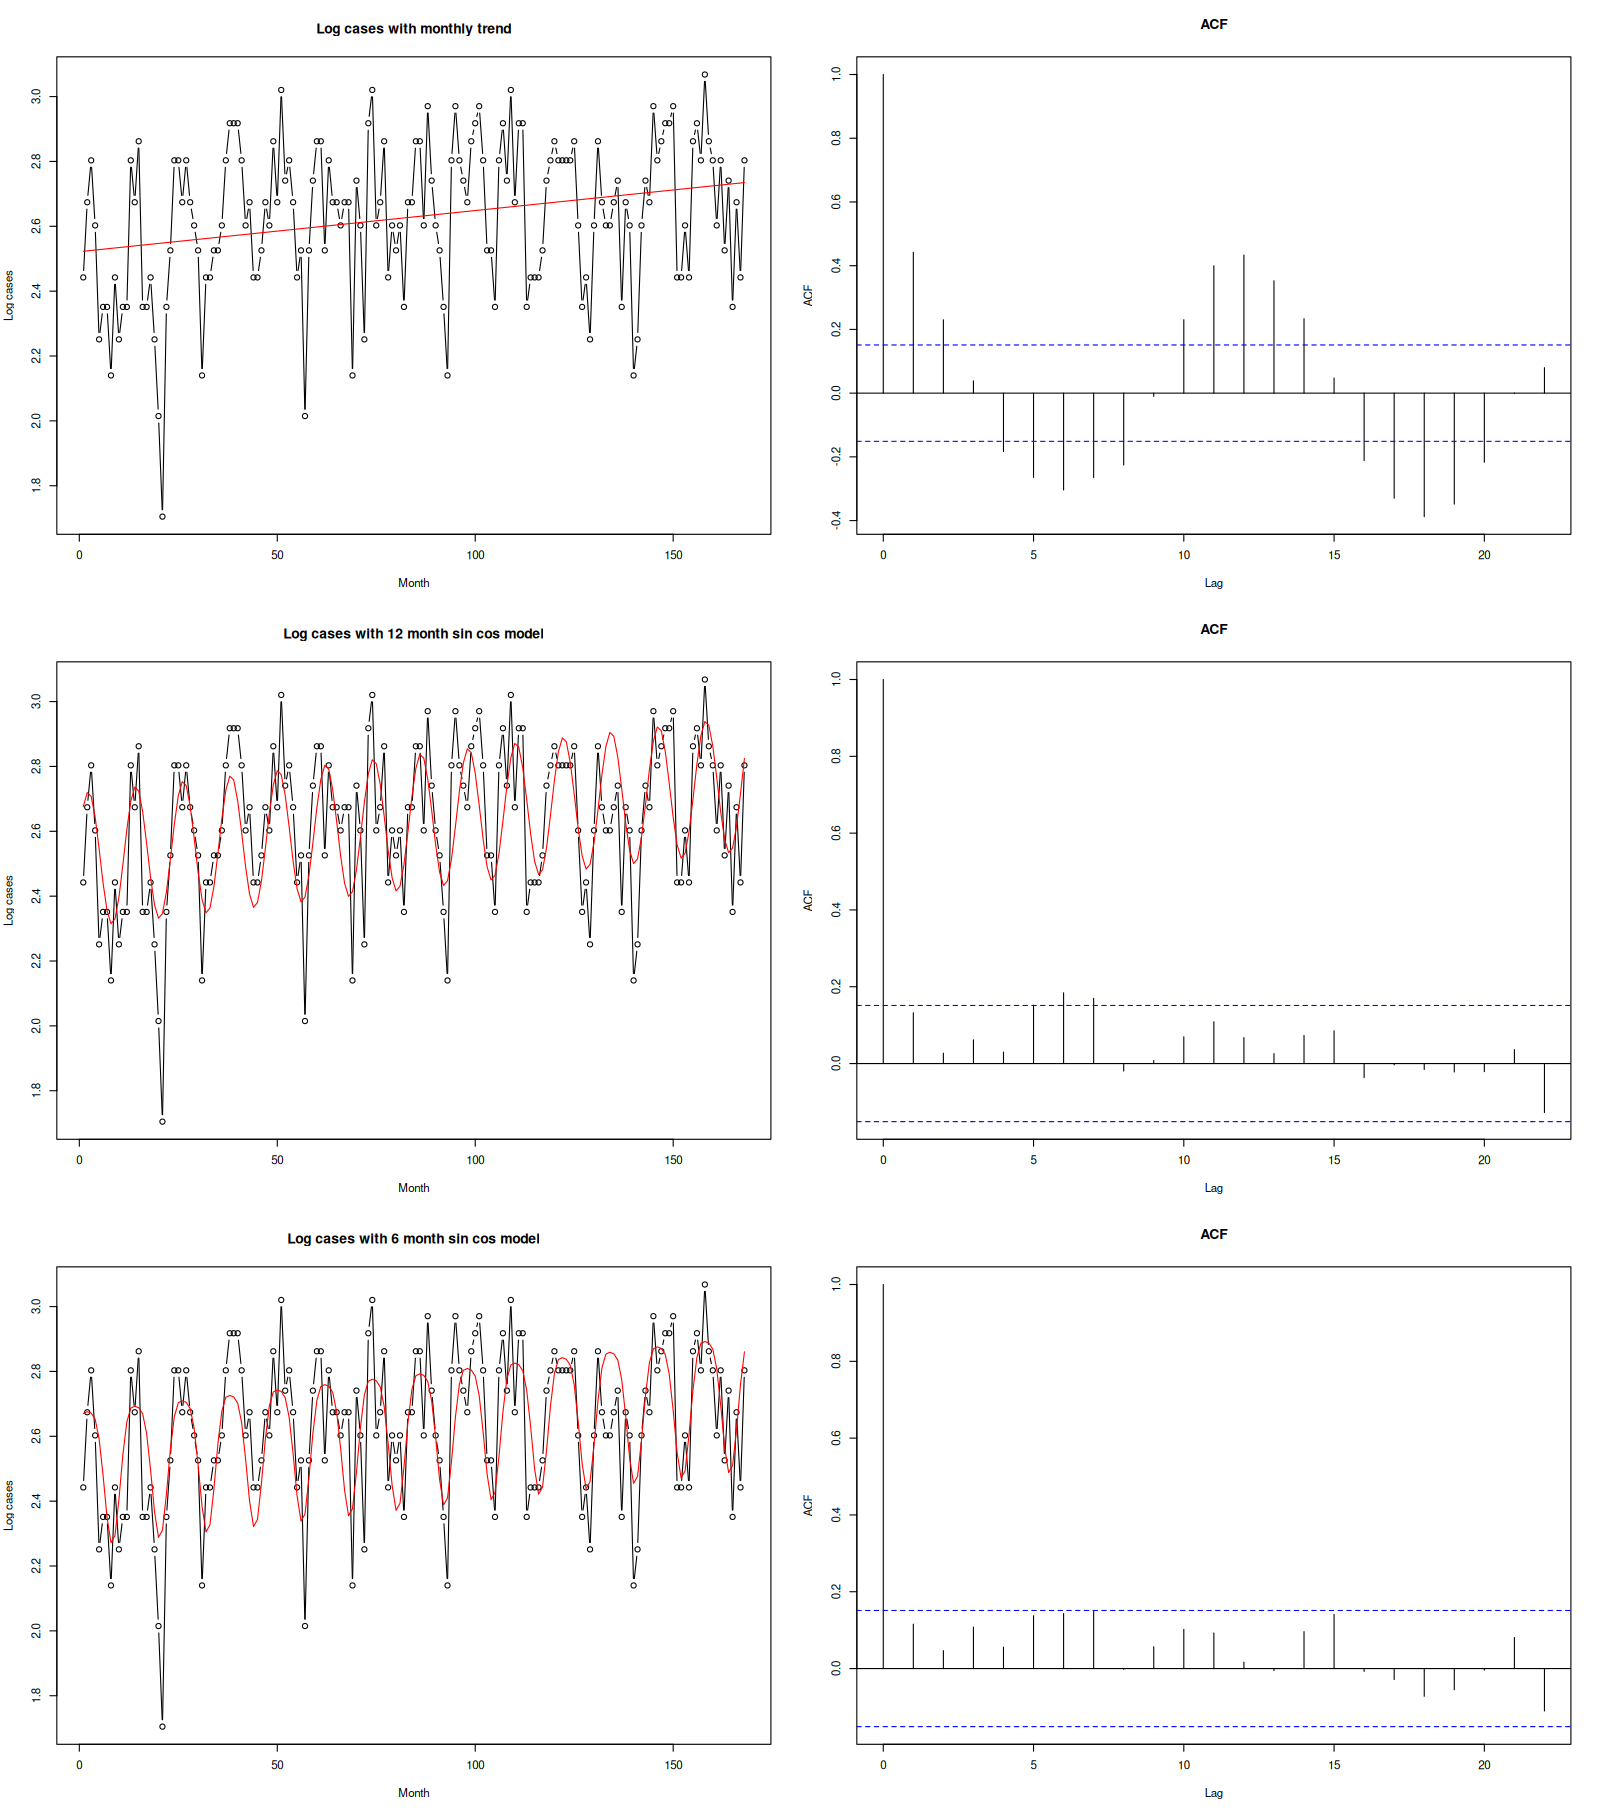
\includegraphics[scale=0.25]{images/sincosmodel.png}
    \caption{Linear models and cases, alongside ACF plots of residuals}
    \label{fig:sincos}
\end{figure}

% validate -> move to arima
So far we have seen that quite a lot of the variance is relatively simple and regular. However, only the general pattern is captured and the fit could be improved with a little more complexity. The biggest issue here is that the covariates which we know are relevant to snakebites, are not included. They cannot simply be added to this model as they themselves have seasonal variation. An alternative model which we can use is the seasonal autoregressive integrated moving average (SARIMA) model. This is proposed next as we have seasonality in our covariates, and we have seen there are autoregressive patterns at various time lags. For brevity we do not go into more detail here about ARIMA models, but a thorough description is given in \cite{damaTimeSeriesAnalysis2021}.

% explain sarima
The SARIMA model was developed to address a limitation of the ARIMA model. Specifically, seasonality is incorporated into the SARIMA model. The ARIMA model is specified using three terms (p,d,q). Depending on the values these take, a specialised case can be applied. For exmaple a moving average ARIMA model would be specified as ARIMA(0,0,q) and an autoregressive model as ARIMA(p,0,0).

SARIMA models have an additional 4 terms to specify the seasonal component. These are (P,D,Q)m. Giving us the following format: SARIMA(p,d,q)(P,D,Q)m. The seasonality period is given as m. P is the number of seasonal autoregressive terms. These terms are sufficient to explore the example snakebite project. Again, for further details one can see \cite{damaTimeSeriesAnalysis2021}.

% define our initial model
A SARIMA model was fit to the data for each region. The model was defined as SARIMA(0,0,0)(1,0,0)12, which is purely a seasonal autoregressive model with a single seasonality component with 12 values per season i.e an annual cycle.

% move some models to sarima + ar1
A number of regions produced residual ACF plots which indicated that an additional term should be introduced. These regions had an additional autoregressive term included with a lag of 1 (AR1). The model for these regions is defined as SARIMA(1,0,0)(1,0,0)12. The residual values after fitting both models to each of these regions is given in Figure \ref{fig:ar1regions}, which shows that the AR1 term was sufficient to capture the remaining temporal autocorrelation/variance. % what word to put here?

% validate and plot
\begin{figure}[h]
    \centering
    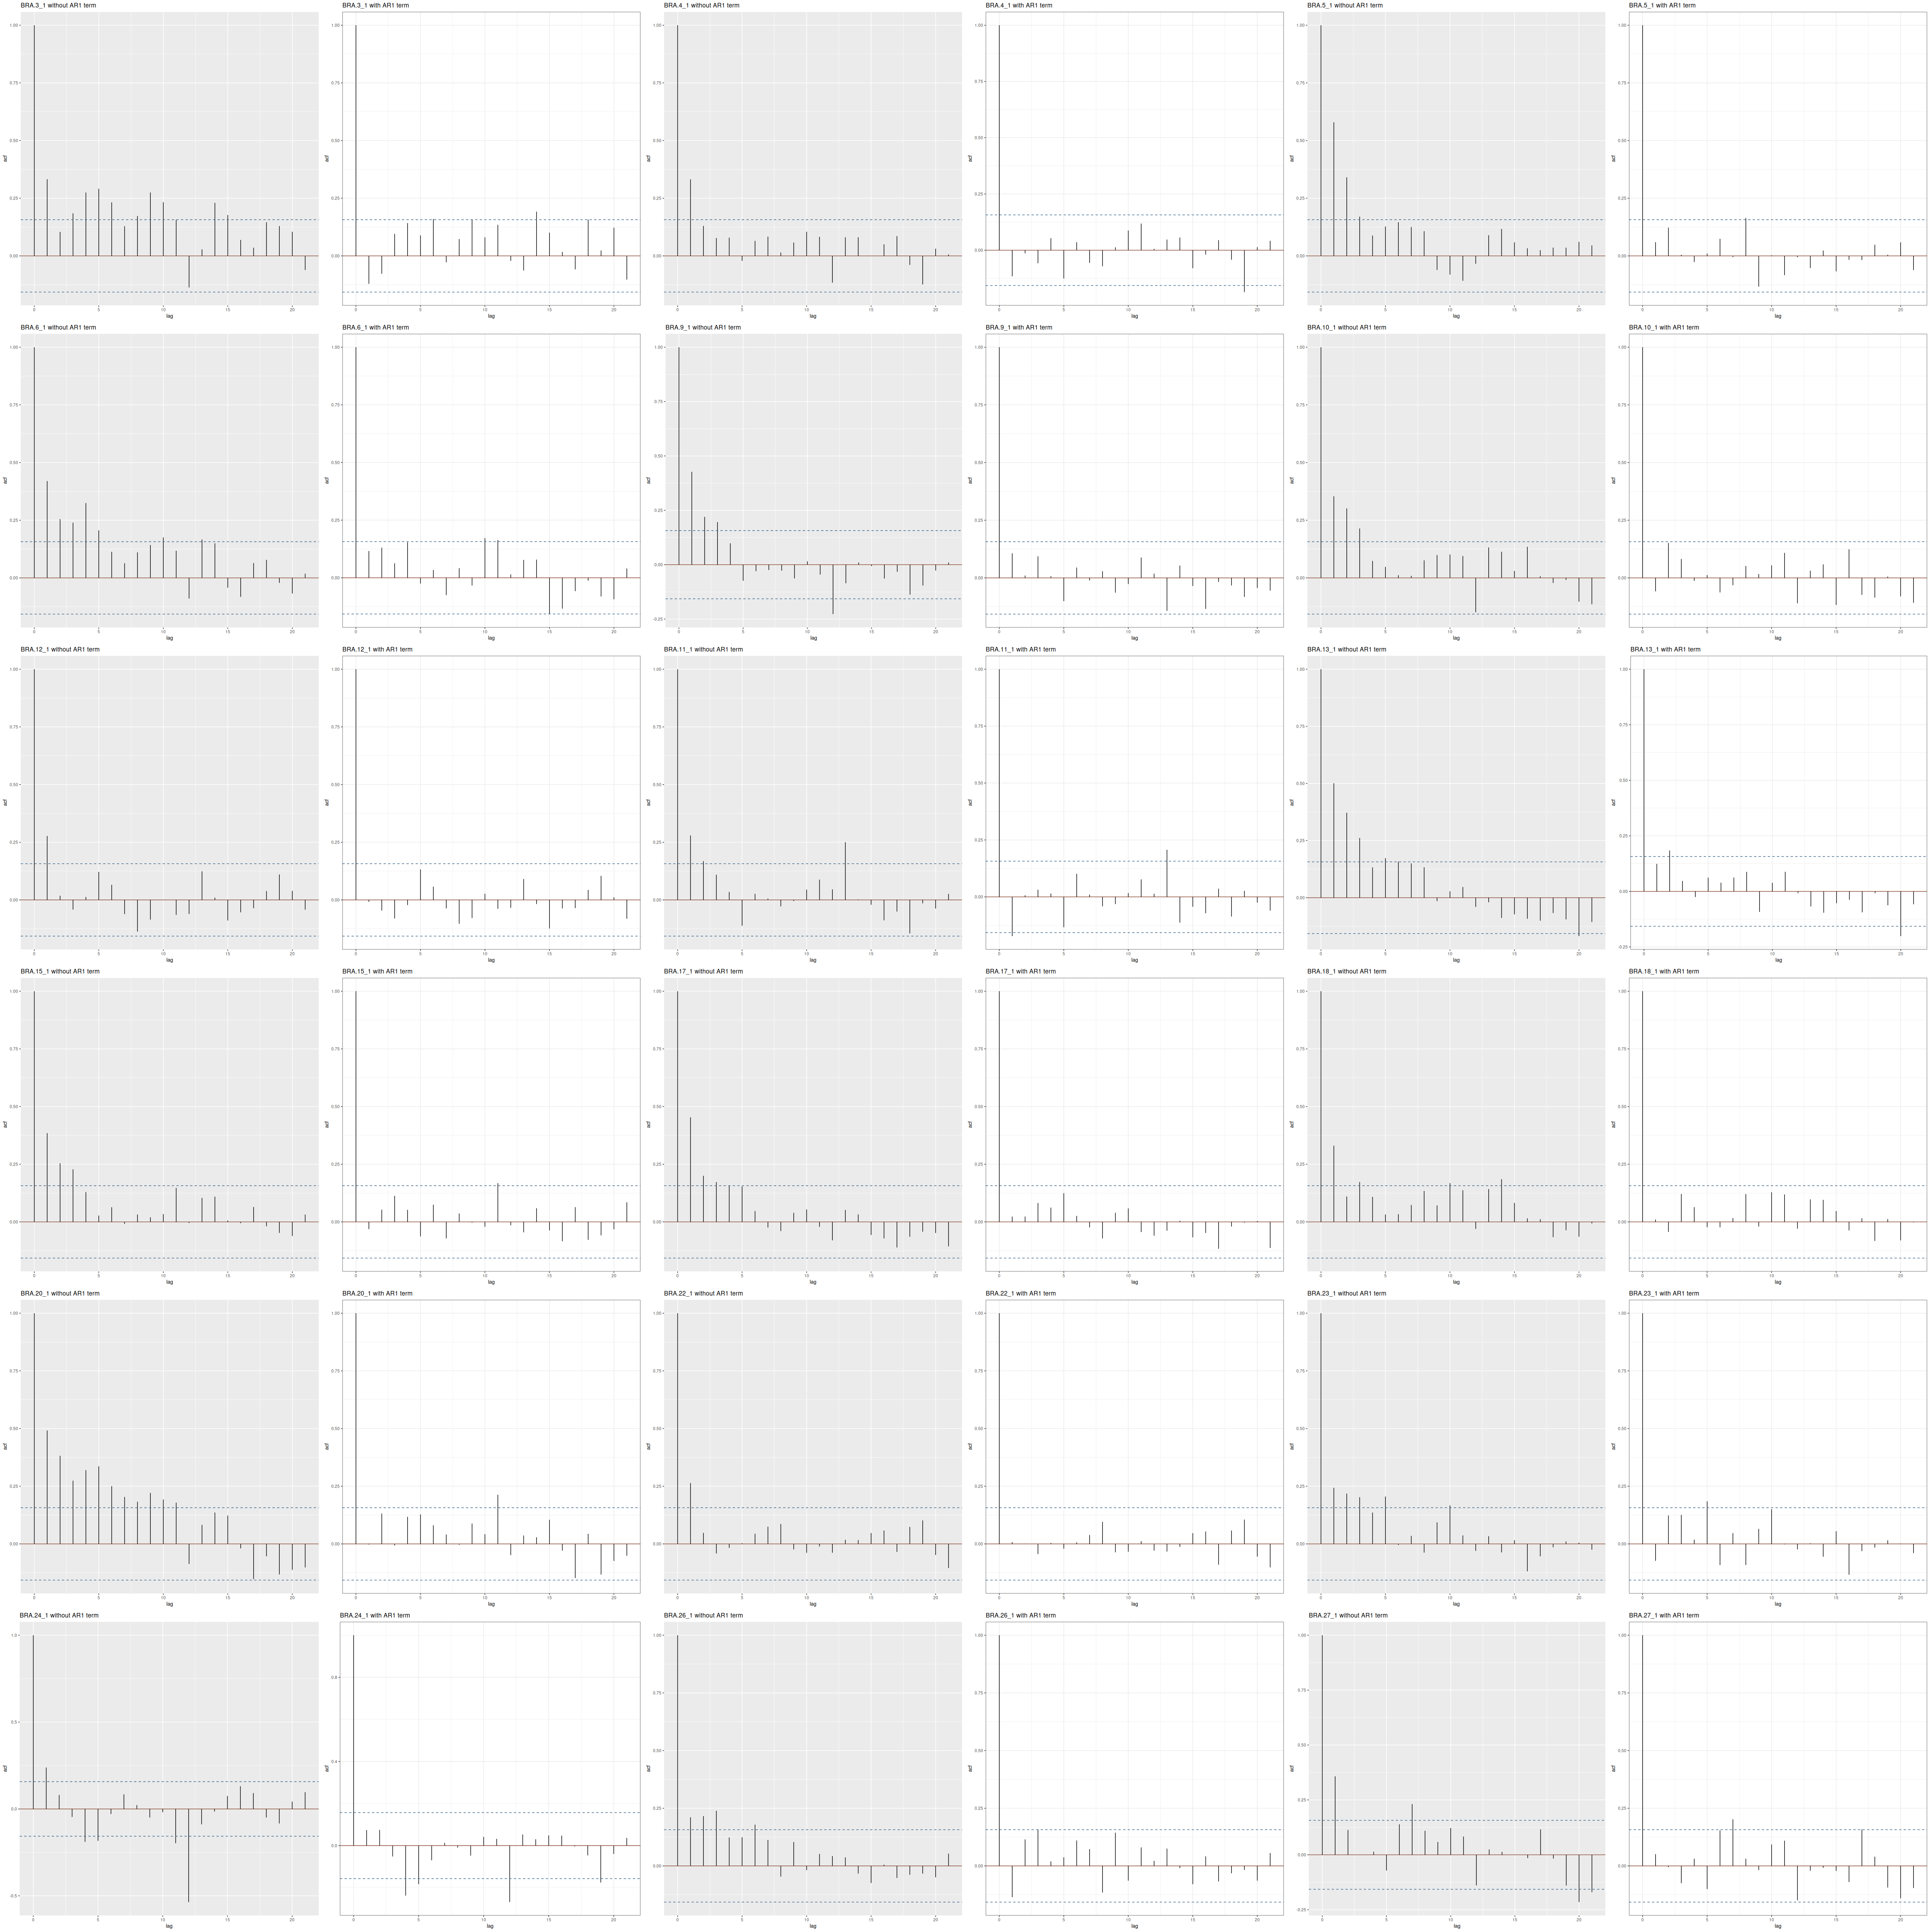
\includegraphics[scale=0.06]{images/ar1regions.png}
    \caption{ACFs of regions identified as needing an additional AR1 term, with and without said term}
    \label{fig:ar1regions}
\end{figure}

Until now each model has included all of the environmental covariates. However, with further propose-validate iterations we can determine which combination of covariates is best for each regions. Here we define best as having the greatest predictive power.

This is part of the parallel process of covariate selection from Figure \ref{fig:framework}, which is intertwined with model development.

% best covariate selection - are any without predictive power. this could be expanded into data mining potentially
When refining the SARIMA model we change the validation to also consider predictive power. This is motivated by our intent to produce projections, deriving from the research questions.

In this case we split the data at a given point into two data sets: test and train. The SARIMA models identified earlier are applied to the test data set. Projections are then produced for these models which overlap with the test data set. The error is then measured and evaluated. In this case, the combination with the lowest error is considered as the best covariate combination for a region.

% general approach - residuals (temporal or other remaining influence)
If our research questions had required the production other outputs then the propose-validate steps would be different. For example, risk maps would be produced by projecting values for other spaces and/or times. These would then be plotted using a criterion such as highlighting locations and times with risk outside of the confidence intervals. Validation could be performed by analysing the residuals of models.

% acceptable performance so predictions done

% IN PARALLEL COVARIATE SELECTION BEST MODEL - DIFFERENT VALIDATION CRITERIA
Each region has its data split by taking the last 2 years of data as the test data set. Each combination of covariates was used to fit the current best SARIMA model to the test data sets. Each combination (including none) was then ranked based on its mean squared error (MSE). Because the size of the data was tractable a full grid search was possible. The best combination of covariates for each region is given in Table \ref{tab:bestcovs}.

\begin{table}
\centering
\caption{Best performing covariate combinations by MSE}
\centering
\begin{tabular}[t]{ll}
\toprule
region & model\\
\midrule
BRA.1\_1 & humidity\\
BRA.2\_1 & rain\\
BRA.3\_1 & none\\
BRA.4\_1 & humidity\_temperature\\
BRA.5\_1 & rain\_temperature\\
\addlinespace
BRA.6\_1 & temperature\_humidity\_rain\\
BRA.7\_1 & none\\
BRA.8\_1 & humidity\\
BRA.9\_1 & humidity\_temperature\\
BRA.10\_1 & none\\
\addlinespace
BRA.12\_1 & temperature\_humidity\_rain\\
BRA.11\_1 & humidity\_temperature\\
BRA.13\_1 & humidity\_temperature\\
BRA.14\_1 & temperature\\
BRA.15\_1 & rain\_temperature\\
\addlinespace
BRA.16\_1 & rain\\
BRA.17\_1 & temperature\_humidity\_rain\\
BRA.18\_1 & temperature\_humidity\_rain\\
BRA.19\_1 & humidity\\
BRA.20\_1 & temperature\_humidity\_rain\\
\addlinespace
BRA.21\_1 & temperature\_humidity\_rain\\
BRA.22\_1 & temperature\_humidity\_rain\\
BRA.23\_1 & temperature\\
BRA.24\_1 & rain\\
BRA.25\_1 & humidity\_temperature\\
\addlinespace
BRA.26\_1 & rain\\
BRA.27\_1 & rain\_temperature\\
\bottomrule
\end{tabular}
\end{table}

% highlight region 8 from graphical results
A graphical representation of the best performing covariate combinations per region is shown in Figure \ref{fig:bestcovs}. The graph makes two things obvious. Firstly, that the best predictive factors for a given region are non-homogenious. Secondly, that region 8 has uniquely large MSE values. This region did not fully participate in reporting cases to SINAN during the time period of the study. The other differences may be due to actual differences in snake distributions and/or snake-human interactions.

\begin{figure}[h]
    \centering
    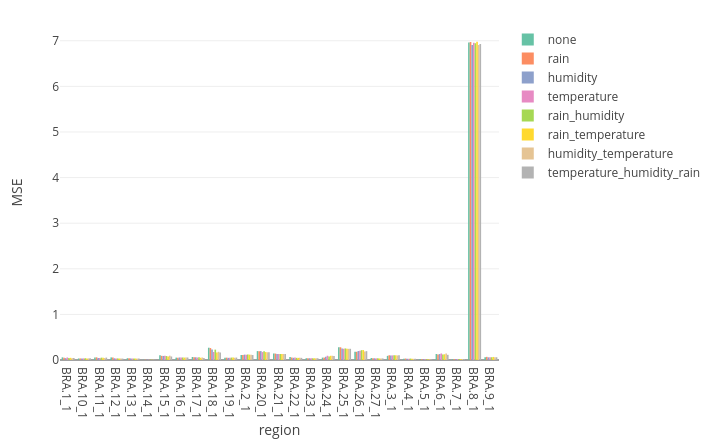
\includegraphics[scale=0.4]{images/bestcovs.png}
    \caption{Mean squared error values for each region-covariates combination.}
    \label{fig:bestcovs}
\end{figure}


% Also mention that the el nino visible, oculd be added, but only visible in monthly means - i.e. weather anomalies. didn't need to add to model, worth mentioning?

% model selection may impose additional processing steps i.e. contiguous id from 1 -> m (number of months) - probably just an implementation detail

% explain how we fit this model - (S)ARIMA - check library, I think it was MLE



\subsection{Outputs}

% I feel like we are still missing this bit. Needs an RQ to focus on, then produce the output and include here
The research questions will largely drive the nature of the outputs from the framework. These often broadly fall in to two categories: Projection and Description.



% Descriptive Mapping 
Descriptive outputs are useful for gaining insights from the data about what the current situation is, where the coverage is sufficient. For example, a map could be produced of regions which have a risk from a particular disease which is above average for a country.

% Projecting
Alternatively, projections can be made. These could take the obvious form of risk maps for future dates i.e. projecting in time. However, this may also be projections in space. An incomplete coverage of data points are used to map out an area; Kriging is an example of this.

% what projections we did

% what the projections can show us - what RQ?

% explain the results

% round up with some conclusions

    % ention that there are constatinst/inputs from lots of sources to elucidate which inform the model and validation, as well as interpretation
\bibliography{snakebites}
\end{document}
